\chapter*{Введение}                         % Заголовок
\addcontentsline{toc}{chapter}{Введение}    % Добавляем его в оглавление

Гетерогенными системами называются системы, имеющие две выделенных роли: host и device. Host это устройство, которое иницирует вычисления и обрабатывает их результаты, device это устройство, на котором производятся вычисления. Обычно хост это микропроцессор (CPU). Исторически именно на CPU запускается операционная система, с которой взаимодействует пользователь. Устройством может быть видеокарточка (GPU), графический ускоритель, специализированная карта для машинного обучения (NPU), другие CPU и даже тот же самый CPU.
\nomenclature{\(CPU\)}{central processing unit, центральный процессор}
\nomenclature{\(GPU\)}{graphics processing unit, видеокарточка}
\nomenclature{\(NPU\)}{neural processing unit, карта машинного обучения}

Исторически первым опытом человечества в гетерогенном программировании были именно видеокарточки.
Созданные как суперпараллельные устройства с фиксированным графическим конвейером и фиксированным набором управляющих состоянием конвейера переключателей, видеокарточки довольно быстро превратились в нечто большее.
Первые короткие программы, позволяющие нетривиальную обработку вершин (после сборки геометрии) и фрагментов (после растеризатора) использовались в основном для освещения и поэтому назывались вершинными и фрагментными \textbf{шейдерами}. Довольно скоро оказалось, что такие шейдеры полезны даже если пропустить собственно рендеринг: в параллельном стиле посчитать что-то на GPU систематически оказывалось быстрее и удобнее чем на CPU \cite{Fang}.

\begin{figure}[ht]
    \centerfloat{
        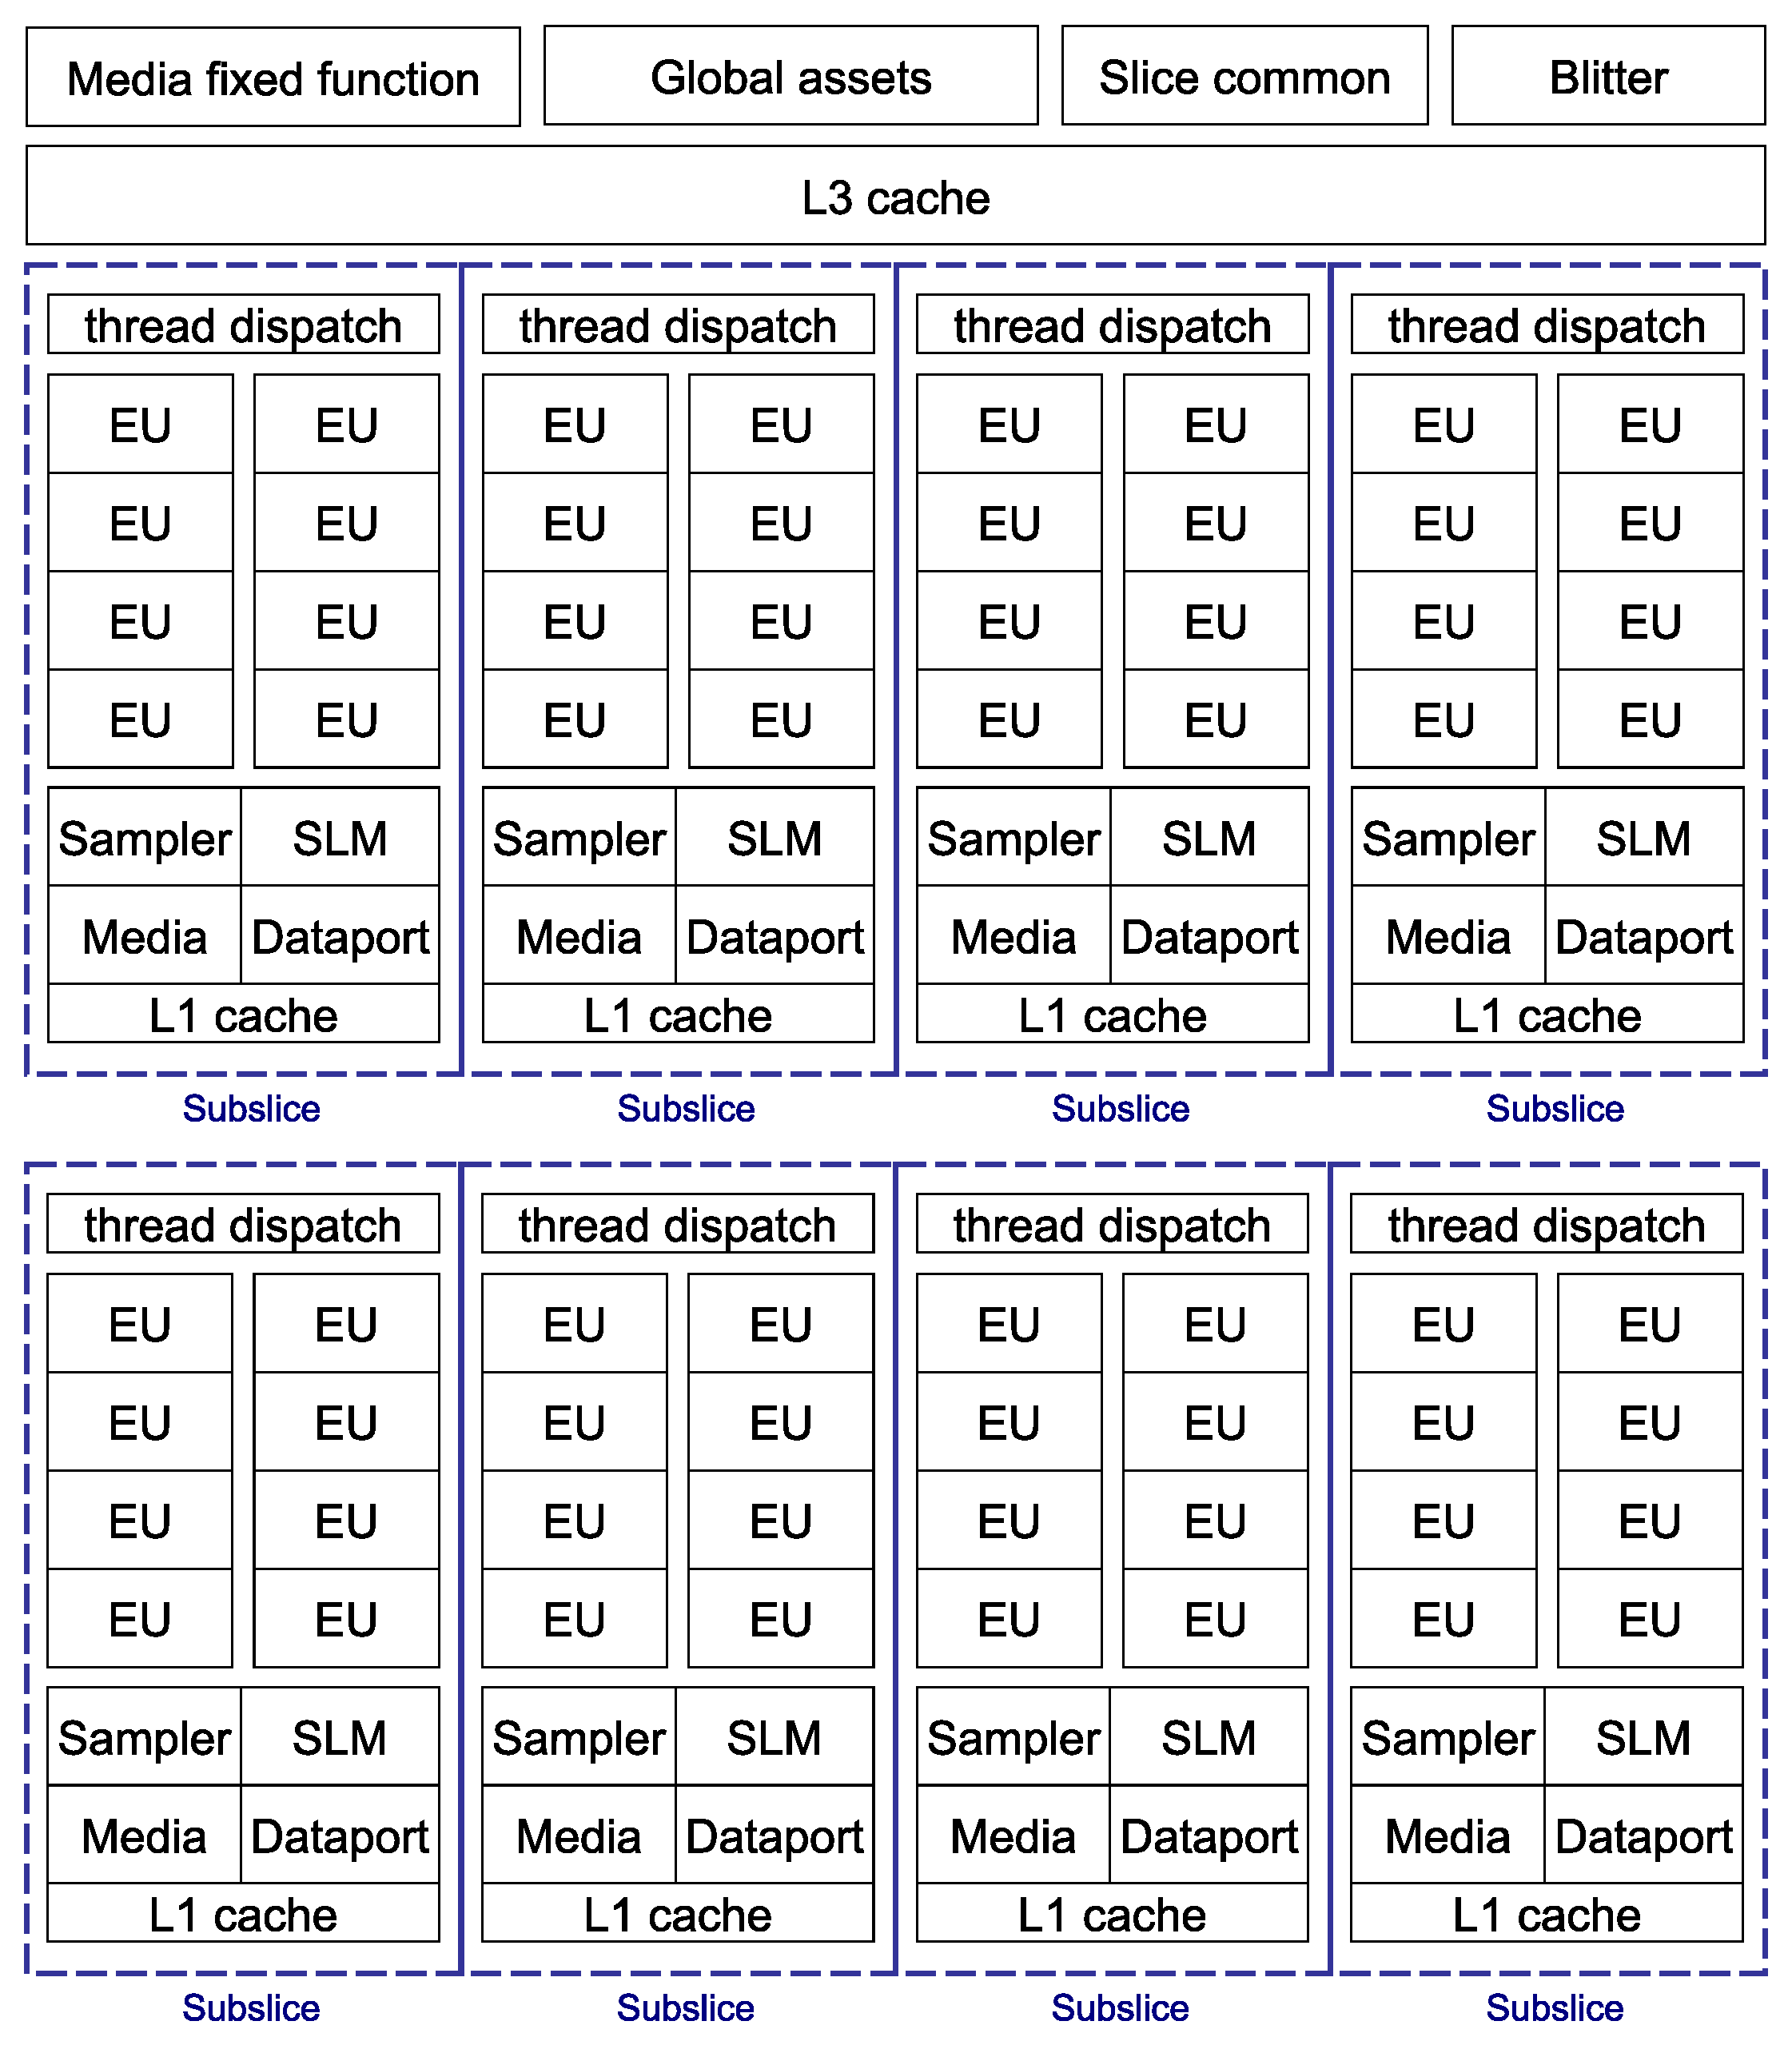
\includegraphics[scale=0.4]{Vladimirov/images/typical-GPU.pdf}
    }
    \caption{Типичное устройство GPU на примере Intel Gen 11}\label{fig:typicalGPU}
\end{figure}

Типичная современная видеокарточка (вариант Intel Gen 11) представлена на рисунке~\cref{fig:typicalGPU}. Можно видеть большое количество параллельных исполнительных устройств, у каждого из которых есть небольшой кеш первого уровня и на всех один общий кеш третьего уровня (второй уровень пропущен конструктивно). Также в каждом подслое (subslice) можно увидеть блок локальной памяти (SLM), Dataport для общения с глобальной памятью, медиаблок и самплер.
\nomenclature{\(SLM\)}{shared local memory, разделяемая локальная память}

Поскольку шейдеры для графики изначально писались не как программы общего назначения а как специализированные программы для конкретных модулей графического конвейера, они писались не на языках общего назначения, а на специализированных языках из которых самыми популярными стали GLSL для OpenGL API и HLSL для DirectX API.

И OpenGL и DirectX и многие более поздние API являются именно API -- то есть набором вызовов, доступных программисту для совершения тех или иных действий. Эти вызовы должны были где-то обрабатываться и формировать запросы к драйверу видеокарточки. Так возникла концепция \textbf{рантайма}, как промежуточного слоя между пользовательской программой и драйвером. Один и тот же рантайм может поддерживать несколько разных API и даже делегировать к нижележащим рантаймам. Например в Intel как OpenCL API так и L0 API поддерживаются одним и тем же NEO runtime (который когда он работает с OpenCL API можно называть OpenCL runtime).

В число поддерживаемых вызовов API неизбежно входит вызов похожий на ``скомпилируй шейдер''. Таким образом неотъемлимой частью рантайма становится \textbf{графический компилятор}.

Первыми опытами в чисто вычислительных задачах исторически стали задачи свёртки (convolution). Именно концепция ядра свёртки (convolution kernel) дала название первым небольшим программам для гетерогенных вычислений: их стали называть \textbf{кернелами}. Ниже везде использование терминов шейдер, кернел и программа будет полностью взаимозаменяемым. В общем нет ошибки в том, чтобы назвать чисто вычислительную программу шейдером и так далее.

\textbf{Целью} данной работы является разработка методов и алгоритмов оптимизации работы с памятью в гетерогенных системах.

Для~достижения поставленной цели необходимо было решить следующие \textbf{задачи}:
\begin{enumerate}[beginpenalty=10000] % https://tex.stackexchange.com/a/476052/104425
  \item Разработать методологию представления высокоуровневых векторных конструкций в векторной системе команд.
  \item Разработать алгоритм разбиения структур данных для улучшения векторизации.
  \item Разработать алгоритм восстановления векторного потока управления.
\end{enumerate}

\iffalse

% TODO: такая структура это хорошая идея но мне пока не хочется портить common

\newcommand{\actuality}{}
\newcommand{\progress}{}
\newcommand{\aim}{{\textbf\aimTXT}}
\newcommand{\tasks}{\textbf{\tasksTXT}}
\newcommand{\novelty}{\textbf{\noveltyTXT}}
\newcommand{\influence}{\textbf{\influenceTXT}}
\newcommand{\methods}{\textbf{\methodsTXT}}
\newcommand{\defpositions}{\textbf{\defpositionsTXT}}
\newcommand{\reliability}{\textbf{\reliabilityTXT}}
\newcommand{\probation}{\textbf{\probationTXT}}
\newcommand{\contribution}{\textbf{\contributionTXT}}
\newcommand{\publications}{\textbf{\publicationsTXT}}

\input{common/characteristic} % Характеристика работы по структуре во введении и в автореферате не отличается (ГОСТ Р 7.0.11, пункты 5.3.1 и 9.2.1), потому её загружаем из одного и того же внешнего файла, предварительно задав форму выделения некоторым параметрам

\textbf{Объем и структура работы.} Диссертация состоит из~введения,
\formbytotal{totalchapter}{глав}{ы}{}{},
заключения и
\formbytotal{totalappendix}{приложен}{ия}{ий}{}.
%% на случай ошибок оставляю исходный кусок на месте, закомментированным
%Полный объём диссертации составляет  \ref*{TotPages}~страницу
%с~\totalfigures{}~рисунками и~\totaltables{}~таблицами. Список литературы
%содержит \total{citenum}~наименований.
%
Полный объём диссертации составляет
\formbytotal{TotPages}{страниц}{у}{ы}{}, включая
\formbytotal{totalcount@figure}{рисун}{ок}{ка}{ков} и
\formbytotal{totalcount@table}{таблиц}{у}{ы}{}.
Список литературы содержит
\formbytotal{citenum}{наименован}{ие}{ия}{ий}.
\fi